\documentclass[12pt]{article}
\usepackage{tasks}
\usepackage{exsheets}
\usepackage{graphicx}
\usepackage{fullpage}
\usepackage{multicol}
\usepackage{amsmath,amsthm,amssymb}
\usepackage{polynom}
\usepackage{setspace}
\usepackage{tikz}
\usetikzlibrary{shapes,arrows}
\SetupExSheets[question]{type=exam}

\usepackage{color}   %May be necessary if you want to color links
\usepackage{hyperref}
\hypersetup{
    %colorlinks=true, %set true if you want colored links
    linktoc=all,     %set to all if you want both sections and subsections linked
    %linkcolor=blue,  %choose some color if you want links to stand out
}

\newtheorem{theorem}{Theorem}
\newtheorem{corollary}{Corollary}[theorem]
\newtheorem{lemma}[theorem]{Lemma}

\newcommand{\N}{\mathbb{N}}
\newcommand{\Z}{\mathbb{Z}}
\newcommand{\R}{\mathbb{R}}

\usepackage{listings}
\usepackage{color}

\definecolor{dkgreen}{rgb}{0,0.6,0}
\definecolor{gray}{rgb}{0.5,0.5,0.5}
\definecolor{mauve}{rgb}{0.58,0,0.82}

% Define block styles
\tikzstyle{decision} = [diamond, draw, fill=blue!20, 
    text width=4.5em, text badly centered, node distance=3cm, inner sep=0pt]
\tikzstyle{block} = [rectangle, draw, fill=blue!20, 
    text width=5em, text centered, rounded corners, minimum height=4em]
\tikzstyle{line} = [draw, -latex']
\tikzstyle{cloud} = [draw, ellipse,fill=red!20, node distance=3cm,
    minimum height=2em]

\lstset{frame=tb,
  language=C++,
  aboveskip=3mm,
  belowskip=3mm,
  showstringspaces=false,
  columns=flexible,
  basicstyle={\small\ttfamily},
  numbers=none,
  numberstyle=\tiny\color{gray},
  keywordstyle=\color{blue},
  commentstyle=\color{dkgreen},
  stringstyle=\color{mauve},
  breaklines=true,
  breakatwhitespace=true,
  tabsize=3
}

\newcommand{\comment}[1]{}

%\linespread{0}

\title{CS246 Midterm Review Notes}
\author{Fall 2019}
\date{Oct 17 2019}

\begin{document}

\maketitle

\tableofcontents
\newpage
\section{Linux Shell}
Shell: interface to the operating system.
\begin{itemize}
    \item Graphical shell: easy to learn but inflexible
    \item Command-line shell: flexible but steep learning curve
\end{itemize}

\comment{
\subsection{History of Shells}
\begin{itemize}
    \item Original was created by Stephen Borne: Borne Shell
    \item Borne Shell was upgraded to Borne Again Shell (Bash)
    \item Other shells: C Shell (csh), Turbo C Shell (tcsh), Korn Shell (ksh)
    
\end{itemize}
}

\subsection{Linux File System}
\begin{itemize}
    \item Files are organized as a tree structure.
    \item The root directory is the root (/) of the file system.
    \item \textbf{Directory:} a file that contains files
    \item \textbf{Path:} Used to specify the location of a file
        \begin{itemize}
            \item E.g. \textbf{/usr/share/dict/words} (first / specifies root directory, other /s are directory separators)
            \item Absolute path: starts at the root file
            \item Relative path: starts relative to the "current directory"
        \end{itemize}
    \item Special directories:
        \begin{itemize}
            \item . - current directory
            \item .. - parent directory
            \item ~ - home directory
            \item \~{}$<$userid$>$ - userid's home directory
        \end{itemize}
\end{itemize}

\subsection{Linux Commands}
Structure of Linux commands: $<$command$>$ $<$arguments$>$
\begin{itemize}
    \item echo \$0 - tells you which shell you are running
    \item bash - switch shell to bash
\end{itemize}

\subsection{Output Redirection}
\begin{itemize}
    \item Output redirection will redirection the output of a program to a file using $>$
    \item $ctrl + d$ tells the cat command that there is no more input, sends an EOF signal, program gets to "react" unlike $ctrl + c$
\end{itemize}

\subsection{Input Redirection}
Input redirection sends input to a program from a file
\begin{itemize}
    \item $cat < file$ - feature of the shell ( shell opens the file and makes content available to the program)
    \item $cat$ $file$ - given a file name, cat finds and opens a file
    \item $cat$ $-n$ $argument <$ $in.txt > out.txt$
\end{itemize}

\subsection{IO Streams}
% put this into a table instead?
\begin{tabular}{c|c|c|c}
     & Standard Input (stdin) & Standard Output (stdout) & Standard Error (stderr) \\\hline
     Default & keyboard & screen & screen\\
     Redirection & Use $<$ to redirect & Use $>$ to redirect & Use 2$>$ to redirect
\end{tabular}

\subsection{Linux Pipes}
A Linux pipe connects stdout of a program to the stdin of another program \\
Note: Using the output of a program as an argument is called \textbf{Embedded Command}
\begin{itemize}
    \item e.g. echo "Today is \$(date) and I am \$(whoami)"
\end{itemize}

\subsection{Wildcard Matching (Globbing Patterns)}
\textbf{Quotes:} Allows embedded commands and suppresses globbing \\
\textbf{Single Quotes:} Does not allow embedded commands and suppresses globbing patterns 
\subsection{Searching within text files}
egrep $<$pattern$>$ $<$file$>$ : extended global regular expression print
\begin{itemize}
    \item looks at one line at a time and outputs lines that match the \textbf{patterns}
    \item Patterns are regular expressions that specify  regular language
    \item egrep is case sensitive
\end{itemize}
\subsection{Regular Expressions}
Regular expressions are only used with egrep and are different from globbing patterns\\\\
    \noindent\begin{tabular}{l|l}
        Symbol & Meaning\\\hline
        a$|$b$|$c$|$d & \text{equivalent to [abcd], "choose one character from the set"} \\ \hline
        \text{[!abcd]} & \text{any 1 character not in the set} \\  \hline
        * & \text{0 or more of the preceding}\\  \hline
        + & \text{1 or more of the preceding} \\  \hline
        ? & \text{0 or 1 occurrences of the preceding} \\  \hline
        . & \text{match any one character} \\  \hline
        .* & \text{match any number of any character} \\  \hline
        $^\wedge pattern$ & \text{force a match to begin at the start of the line} \\ \hline
        $pattern\$$ & \text{force a match to be the last pattern in the line} \\
    \end{tabular}
    \\
Anything written in + can be written with *

\subsection{File Permissions}
Use ls l for a long listing that shows file permissions. \\
Example of file's permissions: $rw\_|r\_x|r\_\_$ (user/owner bits $|$ group bits $|$ other bits)
\begin{itemize}
    \item x for execute. For ordinary files, this means the file can run. For directories, it means you can enter the directory
    \item \textbf{Command to change permissions: } chmod $<$mode$>$ $<$file$>$. How to write the mode:
    \begin{enumerate}
        \item ownership class: \textbf{u}ser, \textbf{g}roup, \textbf{o}ther, \textbf{a}ll
        \item \textbf{+} (add), \textbf{-} (remove) or \textbf{=} (switch)
        \item \textbf{r}, \textbf{w}, or \textbf{x}
    \end{enumerate}
    \item Shortform e.g: \lstinline{chmod 744 file}
\end{itemize}

\section{Shell Scripts}
A shell script is a text file containing a sequence of commands that is executed as a program. 
\begin{itemize}
    \item $\#!/bin/bash$ (shebang line) should appear in every script you write
    \item tells the shell that this is a sequence of bash lines and to "switch to bash" and start executing
\end{itemize}
\subsection{Shell Variables}
\begin{itemize}
    \item Variables contain strings e.g. $x=1$ (no spaces)
    \item Use $\${x}$ to access value
    \item $\$PATH$ gives list of paths
    \item Scripts can be given arguments which is available as variables $\$1$, $\$2$, etc. as the first, second, args respectively
    \item \textbf{Arithmetic operations syntax}: e.g. \$((x+1))
    \begin{itemize}
        \item Bad idea: \$x + 1 because it will give "1 + 1"
    \end{itemize}
\end{itemize}

\subsection{Test Program}
Every process sets a global status code (\$?) which will either by 0 for success or a non-zero for a failure (not just 1 because there are many ways something can fail). \\
A test program evaluates a condition and sets the status code. \\ 
e.g. \lstinline{[ 1 -eq 2 ]} outputs 1. \textbf{Need spaces between because they are arguments}

\subsection{If Statements}
\begin{lstlisting}[language=Bash]
if [ cond ]; then
    # code
elif [ cond ]; then
    # code
else
    # code
fi
\end{lstlisting}

\subsection{While Loop}
\begin{lstlisting}[language=Bash]
while [ cond ]; do
    #code
done
\end{lstlisting}


\subsection{For Loop}
\begin{lstlisting} [language=Bash]
for x in 1 2 3 ... N
do
    #code
done
\end{lstlisting}

%if you want inline code, do \lstinline{code here}
%\lstinline{int x = 5;}

\section{Basic C++}

\textbf{Compiling from the command line:} 
\lstinline{g++ -std=c+14 hello.cc -o myprog} \\
or \lstinline{g++14 hello.cc}
\subsection{C++ I/O Streams}
When you \lstinline{#include <iostream>}, you gain access to 3 global variables.\\
% center this table
\begin{tabular}{l|l|l|l}
     stream & variable & type & code \\ \hline
     stdin & std::cin & istream & cin $>>$ var; \\ \hline 
     stdout & std::cout & ostream & cout $<<$ var; \\ \hline
     stderr & std::cerr & ostream & cerr $<<$ var; \\
\end{tabular}
\begin{itemize}
    \item If a read fails, a default value is used and the program continues (as of C++11). 
    \item It's okay to not initialize a variable as long as you write to it before you read from it
    \item If a read fails, the expression \lstinline{cin.fail()} is tru
    \item If a read fails due to EOF, the \lstinline{cin.fail()} and \lstinline{cin.eof()} are true
    \item An istream variable (cin) can be automatically be converted to a bool.
    \begin{itemize}
        \item \lstinline{cin} is considered true if \lstinline{!cin.fil()}
        \item \lstinline{cin} is false if \lstinline{cin.fail()}
    \end{itemize}
    \item \textbf{Formatting I/O} \lstinline{<iomanip>}
    \begin{itemize}
        \item We use I/O manipulators to change the mode/format of the I/O
        \item e.g \lstinline{ccout << hex << x} : prints in hexadeciamal
        \item \lstinline{ccout << dec;} : back to decimal
        \item Other manipulators include \lstinline{showpoint, setprecision, boolalpha}
    \end{itemize}
\end{itemize}

\subsection{C++ Strings}
\lstinline{#include <string>} Strings in C++ are arrays of characters in memory that is null-terminated\\
\begin{tabular}{l|l}
     comparisons & ==, !=, $<$, $>$   \\ \hline
     concatenations & s1 + s2 \\ \hline
     length & .length() \\ \hline
     access chars & s[i] \\ 
\end{tabular}
\\
\textbf{Reading strings: } 
\begin{itemize}
    \item \lstinline{cin} into a string: read from first non-whitespace char until the first whitespace char
    \item \lstinline{getline(cin, s);}: read until newline
\end{itemize}

\subsection{File I/O Streams}
\lstinline{#include <fstream>}
\begin{itemize}
    \item \lstinline{ifstream} : read from file
    \item \lstinline{ofstream} : write to file
    \item e.g. \lstinline{ifstream file suite.txt}
    \item Anything we can do with an istream variable like cin, we can do with an ifstream variable
\end{itemize}

\textbf{String Stream}
\lstinline{<sstream>} We can use a C++ string as a source/destination for a file using \lstinline{istringstream} and \lstinline{ostringstream}

\subsection{Constants}
Constants are variables whose value cannot be changed.
\begin{lstlisting}
const int n = 5; 
const Node n = {5, nullptr};


int const *p;
p=&n; p=&m; // valid
*p = 5; // not valid


// where the const is changes what can be modified
int * const p;
*p = 5; // valid
p = &n; // no longer valid
\end{lstlisting}

\subsection{References}
C and C++ pass by value.
\begin{lstlisting}
void inc(int n) {
    n += 1;
}
int k = 5;
inc(k);
cout << k; // prints 5
\end{lstlisting}
In C, pointers were used to change values, and addresses were passed. In C++, references are used. References are constant pointers with automatic dereferencing. For example,
\begin{lstlisting}
int y = 5;
int &z = y;
\end{lstlisting}
Whenever \lstinline{z} is written, it means the value pointed at by \lstinline{z}. 
\begin{itemize}
    \item References are also referred to as \textit{alias}.
    \item We cannot have pointers to references
    \begin{itemize}
        \item \lstinline{int &*x = &n;} is wrong
        \item \lstinline{int *&x = something;} is fine
    \end{itemize}
    \item References of an object must be initialized (e.g. \lstinline{int &x;} is wrong)
    \item You cannot have a reference of an array (e.g. \lstinline{int &x=(y,y,y);} is wrong)
    \item \lstinline{int &&x = n;} is wrong since \lstinline{&&} has a different meaning in C++
\end{itemize}

\subsubsection{Pass by Reference}
Although references seems useless since we would usually just use the original, it's good for pass by reference.

\begin{lstlisting}
void inc(int &n) {
    n += 1;
}

int k = 5;
inc(k);
cout << k; // prints 6
\end{lstlisting}

Pass by reference is useful especially when we're passing in very large structs, since we will not need to copy every thing in the struct.

\subsubsection{l-values}

An l-value is:
\begin{itemize}
    \item something that has a permanent place in memory
    \item something that appears on the left hand sign of the assignment operator
    \item something that has a name
    \item E.g. \lstinline{int k = 5;}, \lstinline{k} is an l-value
    \item E.g. \lstinline{2+2} is not an l-value (we can't do \lstinline{int &x = 2 + 2;})
\end{itemize}
With the previous \lstinline{inc()} example, we cannot call \lstinline{inc(2)} as it's written. However, if we pass by const ref, e.g. \lstinline{int inc(const int &n);}, then we can pass in non l-values as well.\\\\
It is strongly recommended that if a parameter does not need to be modified, and is bigger than an \lstinline{int}, pass by const ref. Some trivia, cin passes by const ref.

\subsection{Dynamic Allocation}
\begin{lstlisting}[language=C]
// C style
int *k = malloc(sizeof(int));
free(k)
\end{lstlisting}
\begin{lstlisting}
// C++ style
int *k = new int;
delete k;
\end{lstlisting}
Pointes can be set to nullptr, but refs cannot (called nullable)

\subsection{Operator Overloading}
We can write operator functions, which is useful for custom objects
\begin{lstlisting}
struct Vec {int x, y};
// the motivation is that the + operator should work for Vecs
Vec operator+(const Vec &v1, const Vec &v2) {
    return Vec{v1.x + v2.x, v1.y + v2.y};
}
Vec v{1, 2}, w{3, 4};
v + w; // returns a Vec with 4 and 6

//another example
Vec operator*(int k, const Vec &v1) {
    return Vec{k * v1.x, k * v1.y};
}

Vec operator*(const Vec &v1, int k) {
    return k*v1;
}
\end{lstlisting}

\section{Preprocessors and Compilation}
\subsection{Preprocessors}
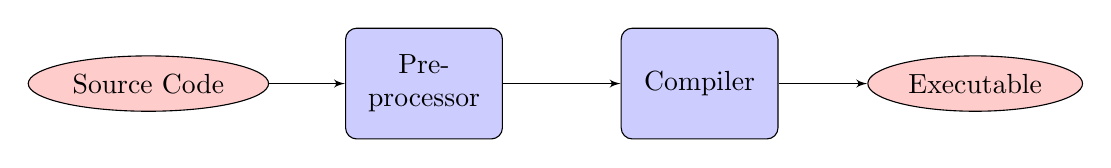
\begin{tikzpicture} [node distance = 3.5cm, auto]
    % Nodes
    \node [cloud] (init) {Source Code};
    \node [block, right of=init] (preprocessor) {Pre-processor};
    \node [block, right of=preprocessor] (compiler) {Compiler};
    \node [cloud, right of=compiler, node distance = 3.5cm] (executable) {Executable};
    % Paths
    \path [line] (init) -- (preprocessor);
    \path [line] (preprocessor) -- (compiler);
    \path [line] (compiler) -- (executable);
\end{tikzpicture}
\\
\lstinline{#include} is a preprocessor directive
\begin{itemize}
    \item Copy and paste the header file
    \item \lstinline{#include <library>} : include from library file
    \item \lstinline{#include "file"} : include from current directory
\end{itemize} 
Other preprocessor directives:
\begin{itemize}
    \item \lstinline{g++ 14 -E file.cc} : shows the outputs of the preprocessor before it goes through the compiler
    \item \lstinline{#define var value} : tells the preprocessor to define var with value using search and replace
        \begin{itemize}
            \item e.g. \lstinline{#define MAX 0} : We can use MAX as a constant
        \end{itemize}
\end{itemize}

\subsection{Conditional Compilation}
\begin{lstlisting}
    #define SECURITY 1 // or 2
    #if SECURITY == 1
        // short int
    #elif SECURITY == 2
        // long long int
    #endif
        // public key
\end{lstlisting}
\begin{lstlisting}
    #define FLAG
    #ifDef VAR // if VAR is defined
        // code
    #endif
    #ifndef VAR // if VAR is NOT defined
        // code
    #endif
\end{lstlisting}
\begin{itemize}
    \item \textbf{Preprocessor variable from the command line}: \lstinline{g++14 -D SECURITY=2 file.cc}
    \item \textbf{Debug variable}: \lstinline{g++ -DEBUG debug.cc}
    \begin{itemize}
        \item compile with the debug variables
        \item recompile with fixes
    \end{itemize}
\end{itemize}

\subsection{Separate Compilation}
Separate compilation breaks programs into :
\begin{enumerate}
    \item Interface files / header files (.h) which includes type definitions and function declarations / prototypes
    \item Implementation files (.cc) which includes function definitions
\end{enumerate}
Separate compilation is for when there are many .cc files.
How to compile: \lstinline{g++14 main.cc vec.cc} \\
\textbf{Never compile header files and never include .cc files}
\\ How to compile main.cc \& vec.cc separately: 
\begin{itemize}
    \item \lstinline{g++ main.cc} : by default, compiler compiles \& produces executable
    \item \lstinline{g++14 -c main.cc} and \lstinline{g++14 -c vec.cc} : gives one compilation
    \begin{itemize}
        \item Produces output file (.o)  \lstinline{g++ main.o vec.o}
        \item When we change one .cc file, we just make one single new object file and them all of them after
    \end{itemize}
\end{itemize}

\subsection{Makefiles}
\textbf{Build tools} keep track of updated files so that we only recompile what is necessary. With Linux, we use \textbf{make}, and we use it by giving a \textbf{Makefile}
A Makefile provides all the dependencies in the program, and is useful for compiling two or more files separately and merging their executables.\\\\
Once the .o files are created, the \lstinline{g++14 main.o otherfile.o ...} will merge the executables. The Makefile is usefule for compiling \textbf{only what is necessary}. Expect to know how to read a Makefile, but knowing how to write one is not necessary for examinations.

\begin{lstlisting}[language=make]
myprogram: main.o vec.o
	g++ main.o vec.o -o myprogram

vec.o: vec.cc vec.h
	g++ -std=c++14 -c vec.cc

main.o: main.cc vec.h
	g++ -std=c++14 -c main.cc
	
filename: dependency dependency
    recipe to make filename

.PHONY: clean

clean:
	rm *.o myprogram
	
//////////////////////////////////////

CXX = g++
CXXFLAGS = -std=c++14 -Wall
OBJECTS = main.o vec.o
EXEC = myprogram

${EXEC}: main.o vec.o
	${CXX} ${CXXFLAGS} ${OBJECTS} -o ${EXEC}

vec.o: vec.cc vec.h

main.o: main.cc vec.h

.PHONY: clean

clean:
	rm ${OBJECTS} ${EXEC}
\end{lstlisting}
% help i dont know where to get notes on this - i have them lol
\subsection{Include Guards}
Oftentimes, multiple files including each other will repeat an include. For example, if file1 includes file2, and both file1 and file2 include file3, nothing would compile. We use include guards to avoid this.
\begin{lstlisting}
#ifndef _VECTOR_H_
#define _VECTOR_H_

struct Vec {
    int x;
    int y;
}

Vec operator+(const Vec &v1, const Vec &v2);

#endif
\end{lstlisting}
Random Note: Never put "using namespace std" in header files.

\section{C++ Classes}
The big idea in Object Oriented Programming (OOP) is that we can put functions in structs.

\begin{lstlisting}
// student.h
# ifndef STUDENT_H
# define STUDENT_H
struct Student {
    int assns, mt, final;
    float grade();
};
#endif

// student.cc
#incldue "student.h"
float Student::grade() {
    return assns * 0.4 + mt * 0.2 + final * 0.4;
}

// main.cc
Student billy{70, 50, 75};
billy.grade()
\end{lstlisting}

\begin{itemize}
    \item In OOP, a class is a struct that contains functions
    \item An instance/value of a class is called an object
    \item A function defined inside a class is called a "member function"/"method"
    \begin{itemize}
        \item Methods can only be called using objects
        \item Methods have access to the fields of the object on which the method was called
        \item Every method has a hidden/automatic parameter. This parameter is called \lstinline{this}
        \item \lstinline{this} is a pointer to the object used to call the method, so \lstinline{this == &billy} or \lstinline{*this == billy}
        \item When accessing fields of the object, we do \lstinline{this->field}
    \end{itemize}
\end{itemize}

\subsection{Object Initialization}
The following are both C-style initialization syntax, which are compile time constant (TODO find out what that means).
\begin{lstlisting}
Student billy{70, 50, 75};
Student billy = {70, 50, 75};
\end{lstlisting}

\subsection{Constructors}
C++ allows writing special methods to construct objects, called constructors. Constructors have no return type, the constructor's name is the class name, and they do not return objects (they construct them)
\begin{lstlisting}
// student.h
struct Student {
    // code
    Student(int assns, int mt, int final);
};
// student.cc
#include "student.h"
Student::Student(int assn, int mt, int final) {
    this->assns = assns;
    this->mt = mt;
    this->final = final;
}
\end{lstlisting}

\subsubsection{Advantages of Constructors}
\begin{itemize}
    \item Constructors are methods, which means they are functions, so constructors get all the nice properties of functions
    \item Arguments need not be compile time constant
    \item Within the constructor body, we can write whatever code we want
    \begin{itemize}
        \item Sanity checks
    \end{itemize}
    \item We can overload constructors
    \item We can put in default arguments
\end{itemize}
\begin{lstlisting}
// student.h
struct Student {
    // code
    Student(int assns = 0, int mt = 0, int final = 0);
    // note that the default values go in the declaration
};

// student.cc
Student::Student(int assns, int mt, int final) {
    this->assns = assns < 0 ? 0 : assns;
    this->mt = mt < 0 ? 0 : mt;
    this->final = final < 0 ? 0 : final;
}

// main.cc
Student s1{70, 60}; // s1.final == 0
Student s2{}; // all fields 0
\end{lstlisting}

\subsection{Default Constructor}
Every class comes with a free default constructor, which is a constructor that takes 0 parameters. 

\begin{itemize}
    \item If you write $any$ constructor yourself, you lose the default constructor as well as C-style initialization.
    \item The default constructor will call constructors on fields that are objects
\end{itemize}
A small example:
\begin{lstlisting}
// MyStruct.h
struct MyStruct {
    int x;
    Student y;
    Vec *z;
};

// main.cc

// this calls the default constructor
MyStruct s;
\end{lstlisting}
The above will compile. \lstinline{x} and \lstinline{z} will not be initialized. \lstinline{y} will be "default" constructed.\\\\

Another example:
\begin{lstlisting}
// Vec.h
struct Vec{
    int x, y;
    Vec(int, int);
};

// Vec.cc
Vec::Vec(int x, int y) {
    this->x = x;
    this->y = y;
}

// main.cc
Vec v{1, 2}; // is not C-style initialization (but it is not)
Vec v1 = {1, 2};
Vec v2; // will not compile since we lost the default constructor
Vec v3 = {1}; // will not work as well
\end{lstlisting}

\subsection{Initializing Fields that are const/lvalue references}
\begin{lstlisting}
int m;
struct MyStruct {
    const int x = m; // in-class initialization (new as of C++11)
    int &y = m;
};

struct Student {
    const int id = 21234567;
    int assns;
    int mt;
    int final;
};
\end{lstlisting}

In this Student example, we would like to initialize the id field and then keep it constant afterwards. To understand how to do this, we must look at how objects are created.

\subsection{Steps of Object Creation}
\begin{enumerate}
    \item Allocate space for the object
    \item Field initialization: default construct fields that are objects
    \item Constructor body runs
\end{enumerate}

The solution is to "hijack" step 2 using member initialization list (MIL)

\subsection{Member Initialization List (MIL)}

\begin{lstlisting}
// student.cc
Student::Student(int id, int assns, int mt, int final) : id{id}, assns{assns}, mt{mt}, final{final} {}
\end{lstlisting}

\begin{itemize}
    \item MIL is only available for constructors
    
    \item MIL can be used to initialize all fields
    \item \lstinline{this} is not required to disambiguate between fields and parameters.
    \item MIL initializes fields in declaration order
    \item MIL can be more efficient than using the constructor body for initializing fields that are objects 
    \item MIL takes precedence over in-class initialization (see example below)
\end{itemize}

\begin{lstlisting}
// vec.h
struct Vec {
    int x = 0;
    int y = 0;
    Vec(int, int);
};

// Vec.cc
Vec::Vec(int x, int y) : x{x}, y{y} {}

// main.cc
Vec v{1, 2}; // the values of x and y are 1 and 2
\end{lstlisting}

\section{The Big 5}

\subsection{Copy Constructors}
Constructing an object as a copy of another object uses the \textbf{copy constructor} 
\begin{lstlisting}
Student billy{70, 50, 75};
Student bobby{billy};
\end{lstlisting}
The copy constructor that comes for free does a field-for-field copy: 
\begin{lstlisting}
Student::Student(const Student &other): assns{other.assns}, mt{other.mt}, final{other.final} {}
\end{lstlisting}
Sometimes this copy constructor is not "correct". For example, with a linked list:
\begin{lstlisting}
// Node.h
struct Node {
    int data;
    Node *next;
    Node(int, Node *);
    Node(const Node &);
};

// Node.cc
Node::Node(int data, Node *next) : data{data}, next{next} {}
Node::Node(const Node &other) : data{other.data}, node{other.next} {} // this is what the free copy constructor would look like

// main.cc
Node *p = new Node{1, new Node {2, new Node {3, nullptr}}};
Node m{*p}; // calling the copy constructor, which is now stack allocated
Node *q = new Node{*p} // same as m, but heap allocated
\end{lstlisting}
%\includegraphics[scale=0.1]{image0.jpeg}\\
The free copy constructor will make a "shallow copy", and all of the lists will share the same nodes.
\begin{itemize}
    \item What happened was that \lstinline{m} created the value 1 correctly, and then copied the $pointer$ to the next node, not the next node
\end{itemize}
We must implement our own constructor to do a "deep copy".
\begin{lstlisting}
Node::Node(const Node &other) : data{other.data}, next{new Node{*other.next}} {}
\end{lstlisting}
The above example creates a new node correctly by recursively calling the copy constructor. However, it is slightly wrong since there is no base case, and we need to handle when other.next is nullptr.
\begin{lstlisting}
Node::Node(const Node &other) : data{other.data}, next{other.next ? new Node{*other.next} : nullptr} {}
\end{lstlisting}

A copy constructor is called whenever
\begin{itemize}
    \item an object is created as a copy of another
    \item there is pass by value - this is the reason why copy constructors are done pass by reference
    \item there is return by value
\end{itemize}

\subsubsection{Constructors with 1 value}
Let's create a function with one parameter.
\begin{lstlisting}
Node::Node(int data) : data{data}, next{nullptr} {}
\end{lstlisting}
One parameter constructors create automatic/implicit conversions. For instance, \lstinline{Node m = 4;} is a valid line of code. If we have a function \lstinline{void foo(Node);}, the line of code \lstinline{foo(4);} is also valid. Another example is \lstinline{string s= "Hello";}. The string constructor has one parameter and implicitly converts the C-style array of characters that is null-terminated into a C++ string. We can disable this automatic conversion by declaring the constructor \lstinline{explicit}.
\begin{lstlisting}
struct Node {
    // code
    explicit Node(int);
};
\end{lstlisting}

\subsection{Destructors}
\begin{itemize}
    \item Stack allocated variables: destroyed when the identifier goes out of the scope.
    \item Heap allocated variables: \lstinline{delete} the pointer to the object
    \begin{itemize}
        \item A method that runs when an object is destroyed (either stack or heap)
    \end{itemize}
    \item The reverse of the 3 steps of object creation:
    \begin{enumerate}
        \item Destructor body runs
        \item Fields are destroyed: destructors are called for fields that objects in reverse declaration order
        \item Memory is deallocated 
    \end{enumerate}
    \item The "free" destructor has an empty destructor body. Sometimes this the wrong thing to do. For example, for a Node struct:
    \begin{lstlisting}
    Node *p = new Node{1, Node{2, new Node{3, nullptr}}};
    delete p;
    \end{lstlisting}
    node 2 and node 3 are not deleted, and thus, we leak memory. We must make our own destructor:
    \begin{lstlisting}
        // Node.h
        struct Node {
            // code
            ~Node();
        };
        
        // Node.cc
        Node::~Node() {
            delete next;
        }
    \end{lstlisting}
\end{itemize}

\subsection{Copy Assignment Operator}
\begin{lstlisting}
Student billy{10, 10, 10};
Student jane = billy;
// this line of code is actually jane.operator=(billy);
\end{lstlisting}
In contrast with the copy constructor, this operator is called when an object is declared, and then assigned the value of another object.\\\\
Example with linked list and nodes:
\begin{lstlisting}
Node &Node::operator=(const Node &other) {
    if (this == &other) return *this // self assignment check
    
    data = others.data
    
    delete next; // we must have this line, since there is an existing object and we have to avoid a memory link
    
    // similar to the copy constructor now
    next = other.next ? new Node {*other.next} : nullptr;
    return *this;
}
\end{lstlisting}
Whenever possible, pass a constant reference. This method should return the updated node and update the node itself. We do this for the same reason we can do this with integers: \lstinline{a = b = c = 0;}. The return type is a reference since it is faster than returning just the object.\\\\
Here is a better implementation:
\begin{lstlisting}
Node &node::operator=(const Node &other) {
    if (this == &other) return *this;
    Node *temp = next; // in case new throws an exception
    next = other.next ? new Node{*other.next} : nullptr;
    
    // if new throws an exception then all the code below will not run
    data = other.data;
    delete temp;
    return *this;
}
\end{lstlisting}

\subsubsection{Copy and Swap Idiom}
\begin{lstlisting}
#include <utility>

struct Node {
    // code
    void swap(Node &);
    Node &operator = (const Node &);
};

void Node::swap(Node &other) {
    using std::swap;
    
    swap(data, others.data);
    swap(next, other.next);
}

Node &Node::operator=(const Node &other) {
    Node tmp{other}; // call the copy constructor
    swap(tmp);
    return *this;
    // we do not have to delete tmp since tmp is stack allocated
}
\end{lstlisting}

\subsection{Move Constructor}
\subsubsection{Rvalues and Rvalue references}
\begin{lstlisting}
Node plusOne(Node n) {
    // code
    return n;
}

Node n{1, new Node{2, nullptr}};
Node n1{plusOne(n)}
\end{lstlisting}
In the above code, \lstinline{n} is passed by value. This calls the copy constructor once initially, and one more time recursively. At the end of \lstinline{plusOne}, it calls the copy constructor (two times again) when returning the value. This returned value "sits" on the right hand side of the assignment temporarily, and then we copy that value (twice again) into \lstinline{n1}. This makes 6 calls in total to the copy constructor.\\\\
An rvalue is:
\begin{itemize}
    \item a temporary
    \item anything not an lvalue
    \item Anything that cannot be referenced, that doesn't have a name, etc.
    \item something that is going to/about to be destroyed
\end{itemize}

The move constructor:
\begin{itemize}
    \item has one parameter, which is an rvalue reference - a reference to an object that is about to be destroyed
    \item Instead of copying from that object, we "steal" their fields since they are going to die anyway
    \item In general, used to construct an object from an rvalue
\end{itemize}

\begin{lstlisting}
Node::Node(Node &&other) : data{other.data}, next{other.next} {
    other.next = nullptr;
}
// we copy with MIL, and the function body deletes the old content
\end{lstlisting}

Recall that an rvalue is a value that has no name, exists momentarily, and is destroyed once it serves its purpose. Note that in the signature of the move constructor, we use the $reference$ of an rvalue.\\\\
Let \lstinline{other} be a reference to an rvalue (say a linked list with 3 nodes). If we ran the copy constructor, it would be less efficient to copy every node of the list. The move constructor instead just copies the first node, and steals the rest, which is more efficient than copying everything.

\subsection{Move Assignment Operator}

Similar to the copy assignment operator, we are assigning to a pre-existing value. Say we have a linked list called \lstinline{l} with nodes 4, 5, 6, and 7. We can swap the values we don't want anymore to the rvalue that is going to be destroyed.
\begin{lstlisting}
Node &Node::operator=(Node &&other) {
    swap(other); // see copy and swap idiom from oct 10
    return *this;
}
\end{lstlisting}

\subsection{Rule of 5}
If you need a custom version of any one of copy constructor, copy assignment operator, desctructor, move constructor, or the move assignment operator, then usually you need all five.

\section{Short Topics}

\subsection{Copy/move Elijsion} 
Turn off -fno-elide-constructors, which would normally skip copying into a temporary value.
\begin{lstlisting}
Vec makeVec() {
    return {1, 2};
}
Vec v1 = makeVec();
\end{lstlisting}
In the code above, the compiler knows where the final resting place of \lstinline{1, 2} and will directly place the values in \lstinline{v1.x} and \lstinline{v1.y}, without calling the copy constructor. C++ allows compilers to elide/avoid calls to copy/move constructors if there is a more efficient way.

\subsection{Overloading Operators}
Should we be implementing operators as methods or stand alone functions?
\\Rules:
\begin{enumerate}
    \item \lstinline{operator=} is implemented as a method. This is because the left hand side will always be referred to as \lstinline{this}
    \item \lstinline{operator[]} must also be implemented as a method
    \item \lstinline{operator()}, \lstinline{operator->}, \lstinline{operatorT()} should be written as methods as well.
\end{enumerate}

\subsection{Arrays of Objects}
How can we write arrays of objects? The below code will not compile.
\begin{lstlisting}
struct Vec {
    int x;
    int y;
    Vec(int, int);
};
Vec arr[10]; // stack array won't compile, no default constructor
Vec *p = new Vec[10]; // heap array won't compile, no default constructor
\end{lstlisting}
Option 1: Write a default constructor\\
Option 2: Stack arrays, explicitly initialize each element
\begin{lstlisting}
Vec arr[3] = {Vec{1, 2}, Vec{3, 4}, Vec{5, 6}}
\end{lstlisting}
Option 3: Use an array of pointers to objects
\begin{lstlisting}
Vec *arr[10];
arr[0] = new Vec{1, 2};

Vec **p = new Vec*[10];
p[i] = new Vec{1, 2};

for (int i = 0; i < 10; ++i) {
    delete p[i];
}
delete [] p;
\end{lstlisting}
\newpage
\subsection{Const Methods}
\begin{lstlisting}
struct Student {
    int assns, mt, final;
    float grade() const {
        return assn * 0.4 + mt * 0.2 + final * 0.4;
    }
};

const Student billy{80, 50, 80};
cout << billy.grade(); // will not work without const on the method name
\end{lstlisting}
The compiler will not allow calling methods on \lstinline{const} objects, even if the method wouldn't change the object's fields anyway. We must append \lstinline{const} to the end of the function declaration, which promises to not change fields of \lstinline{*this}. Note: \lstinline{const} objects can only call \lstinline{const} methods.

\section{Invariants}
\begin{lstlisting}
struct Node {
    int data;
    Node *next;
    ~Node() {delete next;}
};

Node n1{1, new Node {2, nullptr}};
Node n2{3, nullptr};
Node n3{4, &n2};
\end{lstlisting}
The above three nodes will be destructed when they're gone out of scope (they're stack allocated). They will be destroyed with the destructor. Thus, we are attemping to deallocate a stack address, which will crash.\\\\
Node assumed that \lstinline{next} is either \lstinline{nullptr} or points to the heap. When that isn't true, we get undefined behaviour (probably a crash).\\\\
An invariant is a statement/assumption that must be true for code to function correctly. We must prevent the line containing \lstinline{n3} to not compile. In general, we must prevent users from breaking the invariants of our program.

\section{Encapsulation}
\begin{itemize}
    \item Treating objects as capsules/black box.
    \item Implementation is hidden and a few selected methods are exposed.
\end{itemize}

\begin{lstlisting}
struct Vec {
    Vec(int, int); // default visibility is "public"
    private:
    int x, y;
    public:
    Vec operator+(const Vec &rhs) {
        return {x+rhs.x, y+rhs.y};
    }
};
\end{lstlisting}
Note that in the example, we can do \lstinline{rhs.x, rhs.y}. As long as we're within the \lstinline{Vec} code, we can use x and y.
\begin{lstlisting}
int main() {
    Vec v{1,2};
    Vec v1= v + v;
    cout << v.x << v.y; // will not compile, x and y are private
}
\end{lstlisting}
Advice: keep fields private, make select methods public.
\subsection{"Class" keyword}
\begin{itemize}
    \item Default visibility is private
    \item Very similar to struct
\end{itemize}
\begin{lstlisting}
class Vec {
    int x, y;
    public:
    Vec(int,int);
    Vec operator+(const Vec&);
};
\end{lstlisting}
\newpage
\subsection{Node Invariant}
Prevent direct access to Nodes by creating a wrapper List class
\begin{lstlisting}
// list.h
class List {
    struct Node; // declaration of private, nested class
    Node *theList = nullptr;
    public:
    void addToFront(int i);
    int ith(int i);
    ~List();
};

// list.cc
struct List::Node {
    int data;
    Node *next;
    Node(int, Node*);
    ~Node() { delete next; }
};

void List::addToFront(int i) {
    theList = new Node{i, theList};
}

int List::ith(int i) {
    Node *curr = theList;
    for(int j = 0; j < i && curr; ++j,curr=curr->next);
    return curr->data;
}

List::~List() { delete theList; }

///////
List l;
// fill the list with stuff
for (int i = 0; i < n; ++i) {
    cout << l.ith(i);
} // O(n^2) time

Node *curr = theList;
while(curr) {
    // code
    curr = curr->next;
} // O(n) time
\end{lstlisting}

Idea: create an abstraction of a pointer into the list
\begin{lstlisting}
// arr an array
for (int *p = arr; p != arr+size; ++p) {
    ////*p///////
} //TODO: !=, ++, *, begin, end
\end{lstlisting}

\section{Iterator Design Pattern}
Helps us support linear time traversal while still having encapsulation.

\begin{lstlisting}
class List {
    struct Node;
    Node *theList = nullptr;
    public:
    //////
    ////// same methods as before
    
    class Iterator {
        Node *curr
        public:
        Iterator(Node *p) : curr{p} {}
        int &operator*() {
            return curr->data;
        }
        Iterator &operator++() {
            curr = curr->next;
            return *this;
        }
        bool operator!=(const Interator &other) {
            return curr != other.curr;
        }
    };
    Iterator begin() { return Iterator{theList};}
    Iterator end() {return Iterator{nullptr; }}
    
};

\end{lstlisting}
What was the point of this? Now, if we want to traverse the list, this is what we can do:
\begin{lstlisting}
for (List::Iterator it = list.begin(); it != list.end(); ++it) {
    cout << *it << endl; //print 1 2 3 in linear time, and without exposing nodes
    *it += 1; // updates to 2,3,4
}
\end{lstlisting}
We can also use the keyword \lstinline{auto}.

\begin{lstlisting}
for (auto it = list.begin(); it != list.end(); ++it) {
    cout << *it << endl; //print 1 2 3 in linear time, and without exposing nodes
    *it += 1; // updates to 2,3,4
}
\end{lstlisting}
C++ has built in support for the iterator design pattern in the form of what is called Range-based for loops.
\begin{lstlisting}
for (auto &n: list) {
    cout << n; // n is the result of dereferencing
    n += 1;
}
\end{lstlisting}
Note: omtting the \lstinline{&} will create a by value declaration, and will not update curr.

\end{document}